\section{Python Modules for Science}

\subsection{Important tools}

\begin{frame}{The IPython shell}

\begin{exbox}{IPython}
An interactive shell - may replace MatLab [tm] for interactive work
\end{exbox}

\begin{columns}

\column{0.25\textwidth}
\begin{itemize}
    \item Syntax highlighting
    \item Tab completion
    \item Inline documentation
    \item Easy profiling, timing...
    \item IPython $\ge$ 0.11: inline plots...
\end{itemize}

\column{0.75\textwidth}

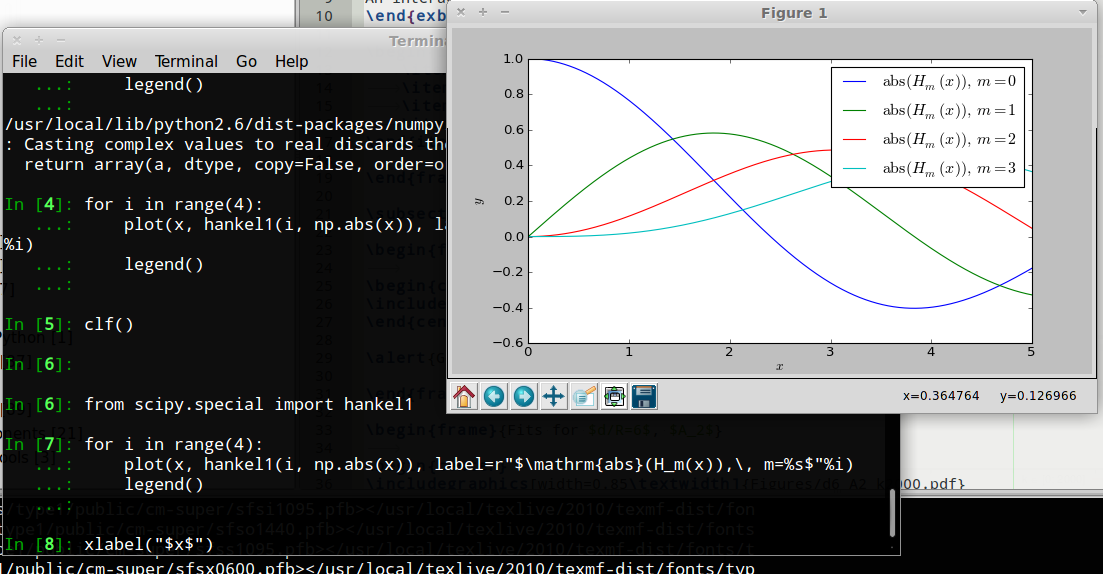
\includegraphics[width=\textwidth]{Figures/Ipython1.png}

\end{columns}

\end{frame}

\subsection{NumPy}

\begin{frame}{NumPy: Python meets an array data type}

\begin{exbox}{NumPy}
Fast and convenient array operations
\end{exbox}

\begin{itemize}
    \item Lists: + does join, not add!
    \item NumPy array: basic vector/matrix data type
    \item Convenience functions (e.g. {\texttt{linspace(), zeros(), loadtxt()...}})
    \item Array slicing
    \item element-wise operations
    \item Code using NumPy reads and writes very similar to modern Fortran
    (slicing, vector valued indices...)
\end{itemize}

\end{frame}

\begin{frame}[fragile]{NumPy by examples}

\begin{Verbatim}[commandchars=\\\{\}]
\PY{k+kn}{import} \PY{n+nn}{numpy} \PY{k+kn}{as} \PY{n+nn}{np}

\PY{n}{a} \PY{o}{=} \PY{n}{np}\PY{o}{.}\PY{n}{array}\PY{p}{(}\PY{p}{[}\PY{l+m+mf}{1.0}\PY{p}{,} \PY{l+m+mf}{2.0}\PY{p}{,} \PY{l+m+mf}{3.0}\PY{p}{,} \PY{l+m+mf}{4.0}\PY{p}{]}\PY{p}{)}
\PY{n}{b} \PY{o}{=} \PY{n}{np}\PY{o}{.}\PY{n}{array}\PY{p}{(}\PY{p}{[}\PY{l+m+mf}{4.0}\PY{p}{,} \PY{l+m+mf}{3.0}\PY{p}{,} \PY{l+m+mf}{2.0}\PY{p}{,} \PY{l+m+mf}{1.0}\PY{p}{]}\PY{p}{)}
\PY{k}{for} \PY{n}{item} \PY{o+ow}{in} \PY{n}{a}\PY{p}{:} \PY{c}{\PYZsh{} arrays are iterable}
    \PY{k}{print}\PY{p}{(}\PY{n}{item}\PY{p}{)}
\PY{n}{c} \PY{o}{=} \PY{n}{a} \PY{o}{+} \PY{n}{b} \PY{c}{\PYZsh{} c = [5, 5, 5, 5]}
\PY{k}{print}\PY{p}{(}\PY{n}{a}\PY{p}{[}\PY{l+m+mi}{0}\PY{p}{:}\PY{l+m+mi}{3}\PY{p}{:}\PY{l+m+mi}{2}\PY{p}{]}\PY{p}{)} \PY{c}{\PYZsh{} 1.0, 3.0; last element not included!}
\PY{n}{a}\PY{p}{[}\PY{l+m+mi}{0}\PY{p}{:}\PY{l+m+mi}{3}\PY{p}{]} \PY{o}{=} \PY{n}{b}\PY{p}{[}\PY{l+m+mi}{0}\PY{p}{:}\PY{o}{-}\PY{l+m+mi}{1}\PY{p}{]}

\PY{k}{print}\PY{p}{(}\PY{n}{a}\PY{o}{*}\PY{n}{b}\PY{p}{)} \PY{c}{\PYZsh{} prints [4, 6, 6, 4], not the scalar product!}
\end{Verbatim}


\end{frame}

\subsection{SciPy}

\begin{frame}{SciPy}

\begin{exbox}{SciPy}
Numerical algorithms using NumPy arrays
\end{exbox}

Wrappers around well-established libraries\\[1.0ex]

Submodules:

\begin{columns}

\column{0.5\textwidth}

\begin{itemize}
    \item {\texttt{linalg}}: linear algebra (lapack)
    \item{\texttt{sparse}}: sparse matrices
    \item {\texttt{fft}}: FFT (fftpack)
    \item {\texttt{optimize}}: optimization, zeros (minpack)
\end{itemize}


\column{0.5\textwidth}

\begin{itemize}
    \item {\texttt{integration}}: integration (quadpack, odepack)
    \item {\texttt{special}}: special functions (amos...)
    \item {\texttt{signal}}: signal processing
\end{itemize}

\end{columns}

\end{frame}

\begin{frame}[fragile]{SciPy: an example}

\begin{Verbatim}[commandchars=\\\{\}]
\PY{k+kn}{import} \PY{n+nn}{numpy} \PY{k+kn}{as} \PY{n+nn}{np}
\PY{k+kn}{from} \PY{n+nn}{scipy.optimize} \PY{k+kn}{import} \PY{n}{curve\PYZus{}fit}
\PY{k+kn}{from} \PY{n+nn}{matplotlib.pyplot} \PY{k+kn}{import} \PY{n}{plot}\PY{p}{,} \PY{n}{show}\PY{p}{,} \PY{n}{legend}

\PY{n}{x}\PY{p}{,} \PY{n}{yExp} \PY{o}{=} \PY{n}{np}\PY{o}{.}\PY{n}{loadtxt}\PY{p}{(}\PY{l+s}{"}\PY{l+s}{func.dat}\PY{l+s}{"}\PY{p}{,} \PY{n}{unpack}\PY{o}{=}\PY{n+nb+bp}{True}\PY{p}{)}
\PY{n}{plot}\PY{p}{(}\PY{n}{x}\PY{p}{,} \PY{n}{yExp}\PY{p}{,} \PY{n}{ls}\PY{o}{=}\PY{l+s}{"}\PY{l+s}{--}\PY{l+s}{"}\PY{p}{,} \PY{n}{c}\PY{o}{=}\PY{l+s}{"}\PY{l+s}{blue}\PY{l+s}{"}\PY{p}{,} \PY{n}{lw}\PY{o}{=}\PY{l+s}{"}\PY{l+s}{1.5}\PY{l+s}{"}\PY{p}{,} \PY{n}{label}\PY{o}{=}\PY{l+s}{"}\PY{l+s}{Exp.}\PY{l+s}{"}\PY{p}{)}

\PY{k}{def} \PY{n+nf}{fitFunc}\PY{p}{(}\PY{n}{x}\PY{p}{,} \PY{n}{a}\PY{p}{,} \PY{n}{b}\PY{p}{,} \PY{n}{c}\PY{p}{)}\PY{p}{:}
    \PY{k}{return} \PY{n}{a}\PY{o}{*}\PY{n}{np}\PY{o}{.}\PY{n}{exp}\PY{p}{(}\PY{o}{-}\PY{n}{b}\PY{o}{*}\PY{n}{x}\PY{p}{)} \PY{o}{+} \PY{n}{c}

\PY{n}{pOpt}\PY{p}{,} \PY{n}{pCov} \PY{o}{=} \PY{n}{curve\PYZus{}fit}\PY{p}{(}\PY{n}{fitFunc}\PY{p}{,} \PY{n}{x}\PY{p}{,} \PY{n}{yExp}\PY{p}{)}
\PY{n}{yFit} \PY{o}{=} \PY{n}{fitFunc}\PY{p}{(}\PY{n}{x}\PY{p}{,} \PY{n}{a}\PY{o}{=}\PY{n}{pOpt}\PY{p}{[}\PY{l+m+mi}{0}\PY{p}{]}\PY{p}{,} \PY{n}{b}\PY{o}{=}\PY{n}{pOpt}\PY{p}{[}\PY{l+m+mi}{1}\PY{p}{]}\PY{p}{,} \PY{n}{c}\PY{o}{=}\PY{n}{pOpt}\PY{p}{[}\PY{l+m+mi}{2}\PY{p}{]}\PY{p}{)}
\PY{n}{plot}\PY{p}{(}\PY{n}{x}\PY{p}{,} \PY{n}{yFit}\PY{p}{,} \PY{n}{label}\PY{o}{=}\PY{l+s}{"}\PY{l+s}{Fit: \PYZdl{}a = }\PY{l+s+si}{\PYZpc{}s}\PY{l+s}{; b = }\PY{l+s+si}{\PYZpc{}s}\PY{l+s}{; c= }\PY{l+s+si}{\PYZpc{}s}\PY{l+s}{\PYZdl{}}\PY{l+s}{"}\PYZbs{}
     \PY{o}{\PYZpc{}}\PY{p}{(}\PY{n}{pOpt}\PY{p}{[}\PY{l+m+mi}{0}\PY{p}{]}\PY{p}{,} \PY{n}{pOpt}\PY{p}{[}\PY{l+m+mi}{1}\PY{p}{]}\PY{p}{,} \PY{n}{pOpt}\PY{p}{[}\PY{l+m+mi}{2}\PY{p}{]}\PY{p}{)}\PY{p}{,} \PY{n}{ls}\PY{o}{=}\PY{l+s}{"}\PY{l+s}{-}\PY{l+s}{"}\PY{p}{,} \PY{n}{lw}\PY{o}{=}\PY{l+s}{"}\PY{l+s}{1.5}\PY{l+s}{"}\PY{p}{,} \PY{n}{c}\PY{o}{=}\PY{l+s}{"}\PY{l+s}{r}\PY{l+s}{"}\PY{p}{)}
\PY{n}{legend}\PY{p}{(}\PY{p}{)}\PY{p}{;} \PY{n}{show}\PY{p}{(}\PY{p}{)}
\end{Verbatim}


\end{frame}

\begin{frame}{SciPy: the example's output}

\begin{center}
    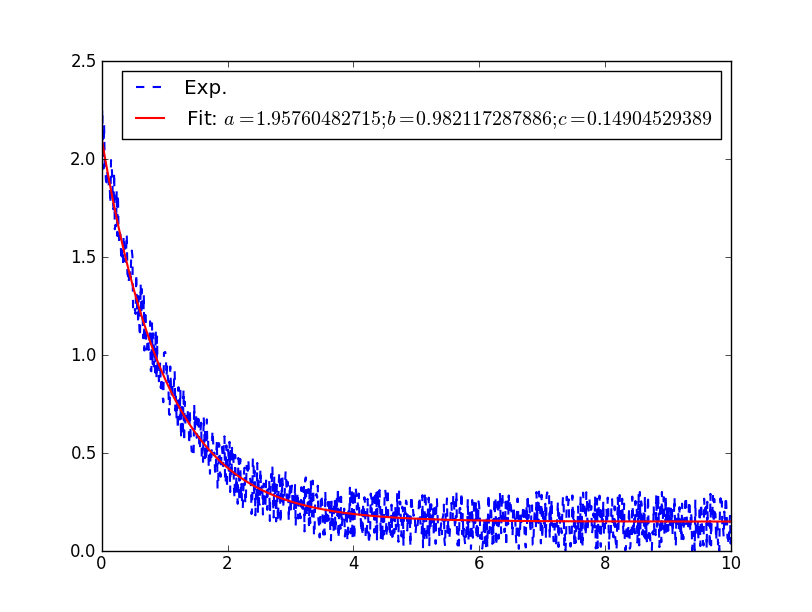
\includegraphics[width=0.8\textwidth]{Figures/fit-png}
\end{center}

Already used here: \emph{Matplotlib}

\end{frame}

\subsection{Matplotlib}

\begin{frame}{Matplotlib}

(mostly) 2D plots

\begin{center}
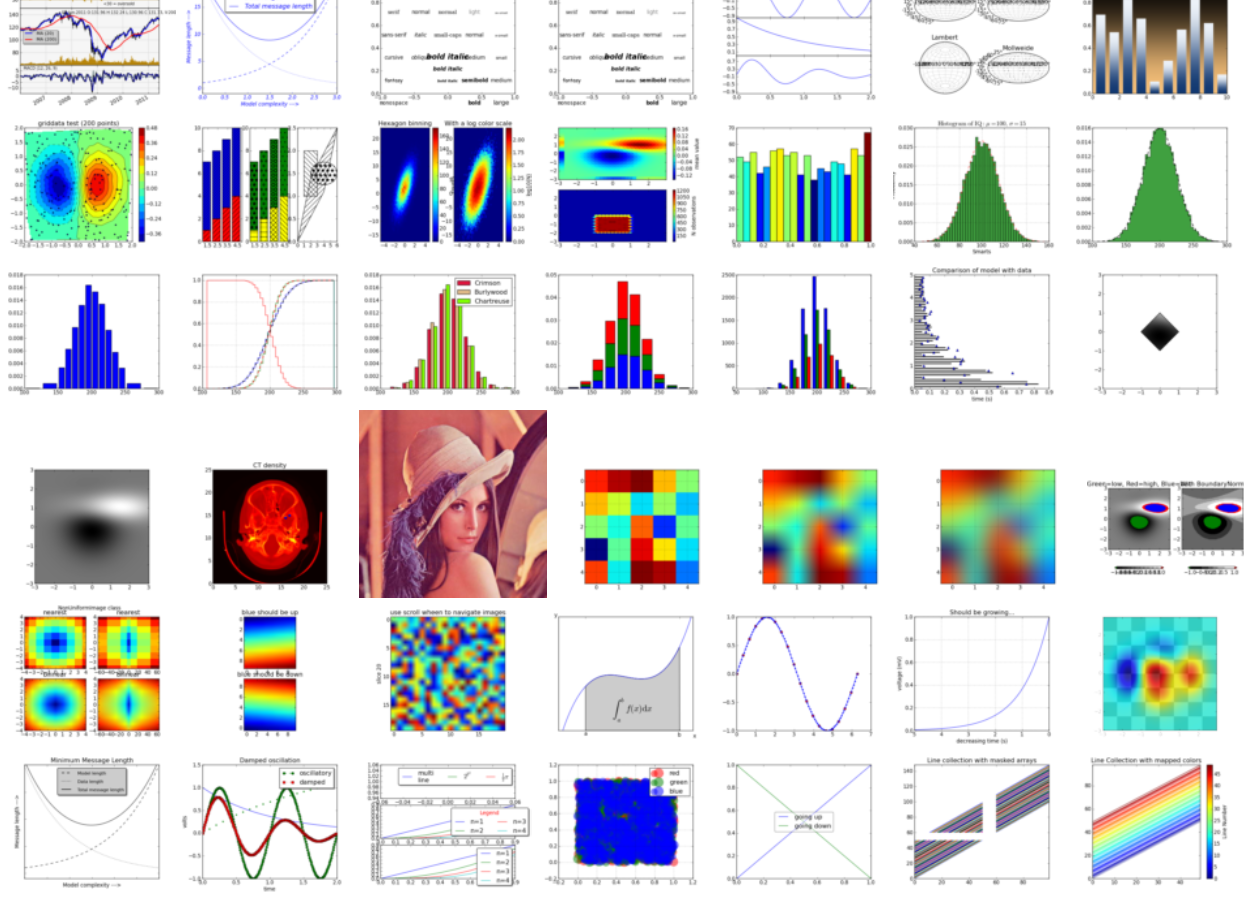
\includegraphics[width=0.8\textwidth]{Figures/mpl}
\end{center}

Pylab: MatLab alternative for interactive work
\end{frame}


\begin{frame}{Some Pylab: the logistic map $x_{n+1}= rx_n(1-x_n)$}
\input{Pygsnippets/logMap.tex}
\end{frame}

\begin{frame}{Some Pylab: the logistic map $x_{n+1}= rx_n(1-x_n)$}

The last script produces this image:

\begin{center}
    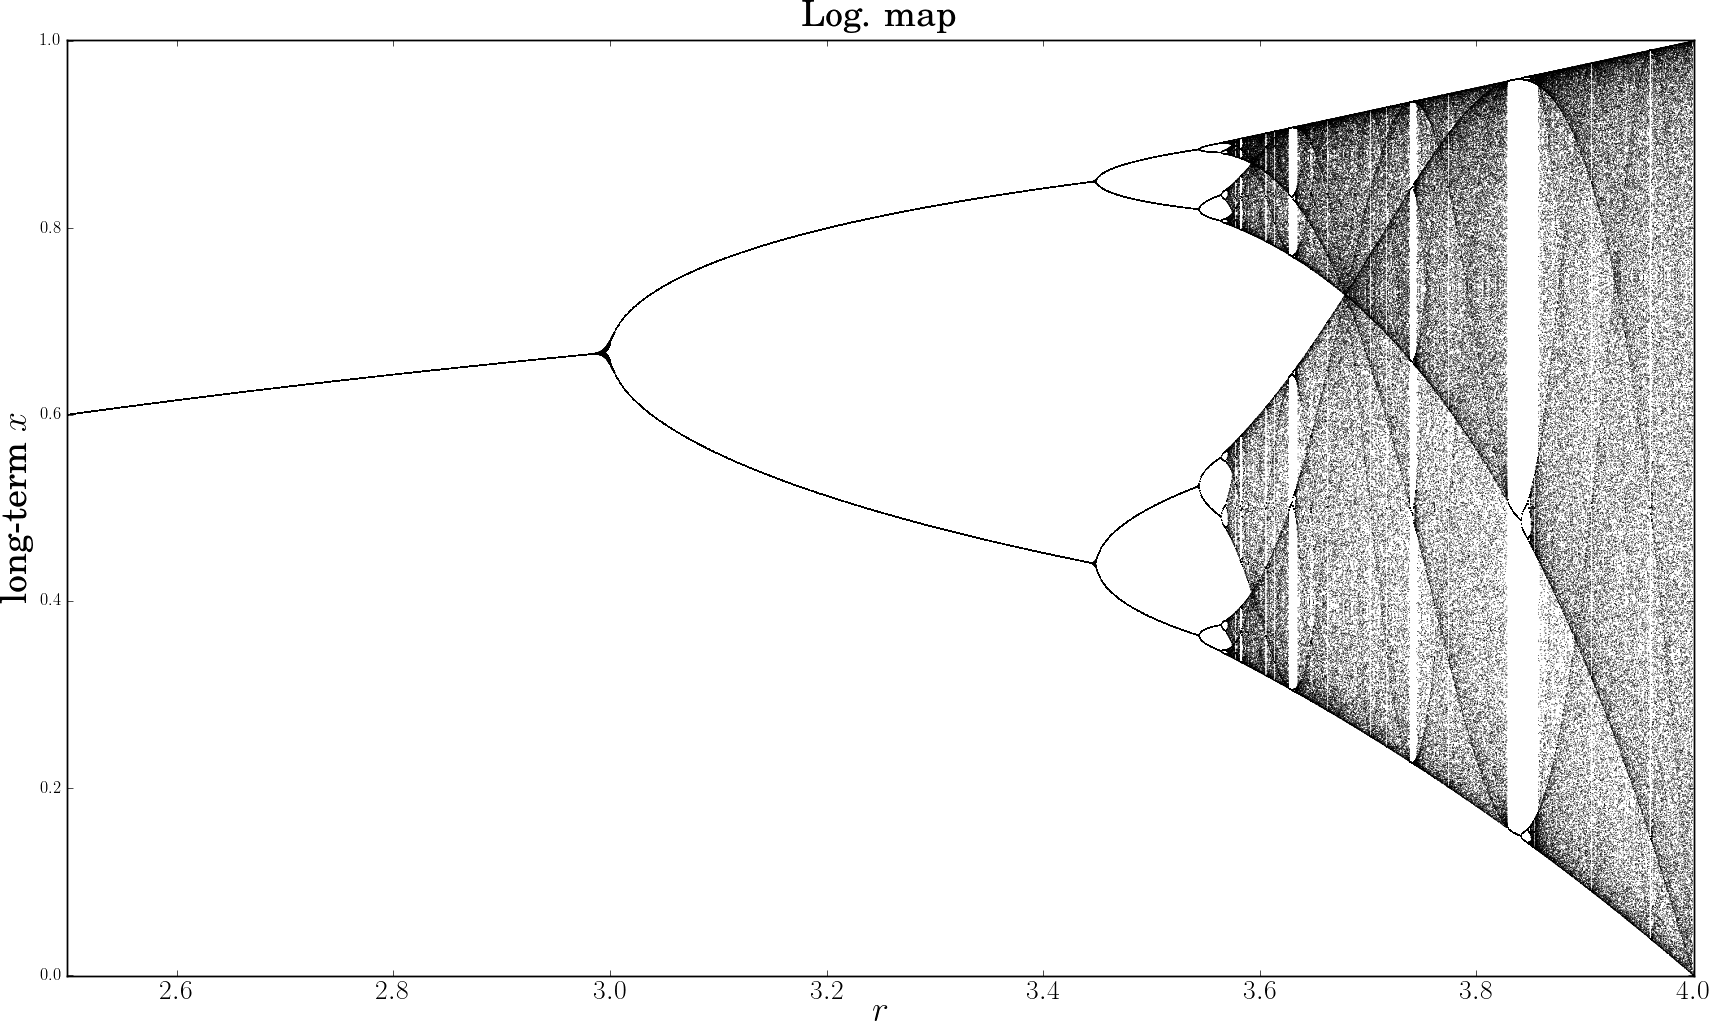
\includegraphics[width=0.9\textwidth]{Figures/logMap}
\end{center}

\end{frame}
